\section{Use Case: GtoPdb}
\label{section:use_case}

\begin{figure}[t]
\centering
  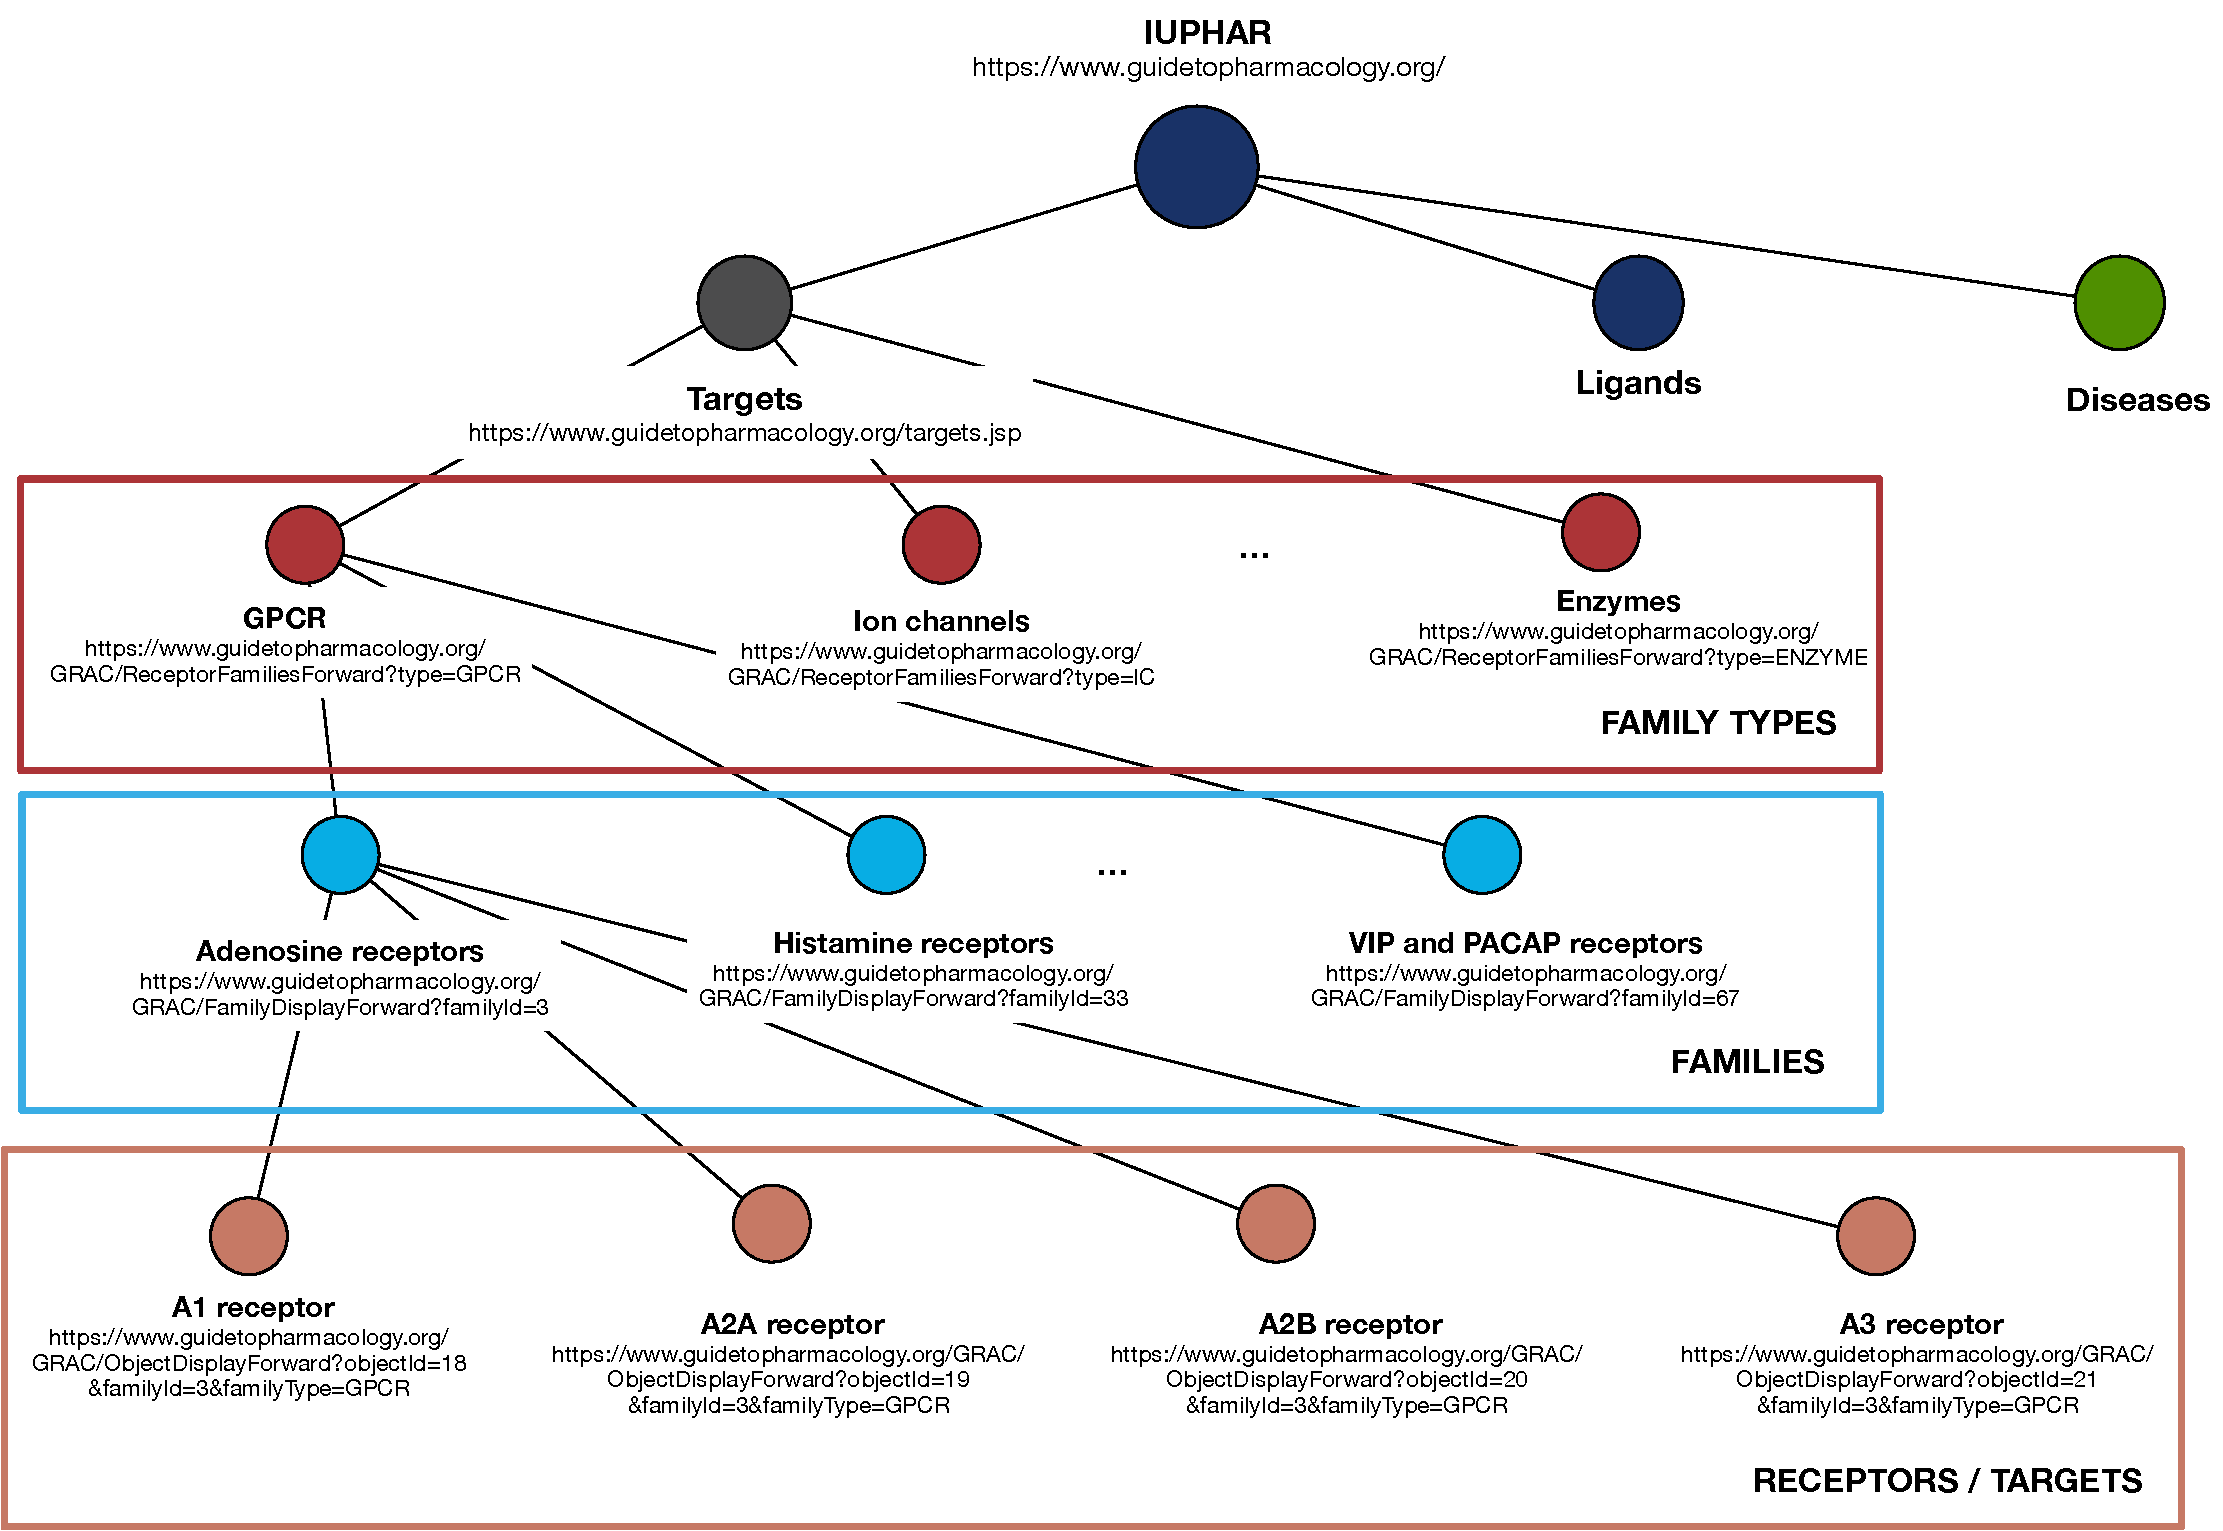
\includegraphics[width=.9\textwidth]{figures/iuphar_schema}
  \caption{Partial map of the GtoPdb hierarchical structure grouping the targets into families and family types.}
  \label{figure:iuphar_schema}
\end{figure}

The IUPHAR/BPS Guide to Pharmacology \citep{iuphar2018}  (GtoPdb\footnote{\url{https://www.guidetopharmacology.org/}}) is a well-known and well structured scientific relational database that contains expertly curated information about diseases, drugs in clinical use, their cellular targets, and the mechanisms of action on the human body. 
It is curated and maintained by the GtoPdb Committee and 96 subcommittees, comprising 512 scientists collaborating with in-house curators who draw the information contained in the database from high-quality pharmacological and medicinal chemistry literature.
Roughly $1000$ researchers from all over the world have contributed to the database, and the curators wanted to give recognition to these contributors.  This led to some early work on data citation~\citep{buneman2006cite}.  

GtoPdb is relational, but its logical structure is hierarchical as shown in Figure \ref{figure:iuphar_schema}.  The information contained in the database is also organized into webpages focused on specific diseases, targets or ligands, and families % (i.e., groups) of them 
for easier access by users. 
As depicted in Figure \ref{figure:iuphar_schema}, the database can be thought of as a tree where the root is the database; the first level consists of all targets, ligands, and diseases; and the lower levels consists of specific targets, ligands and diseases. 
In this paper, we focus on targets; thus the figure at the third level shows examples of family types, at the fourth level of specific families of targets (a finer level of granularity), and finally, at the last level, the single targets (also known as receptors). 

\begin{figure}[t]
\centering
  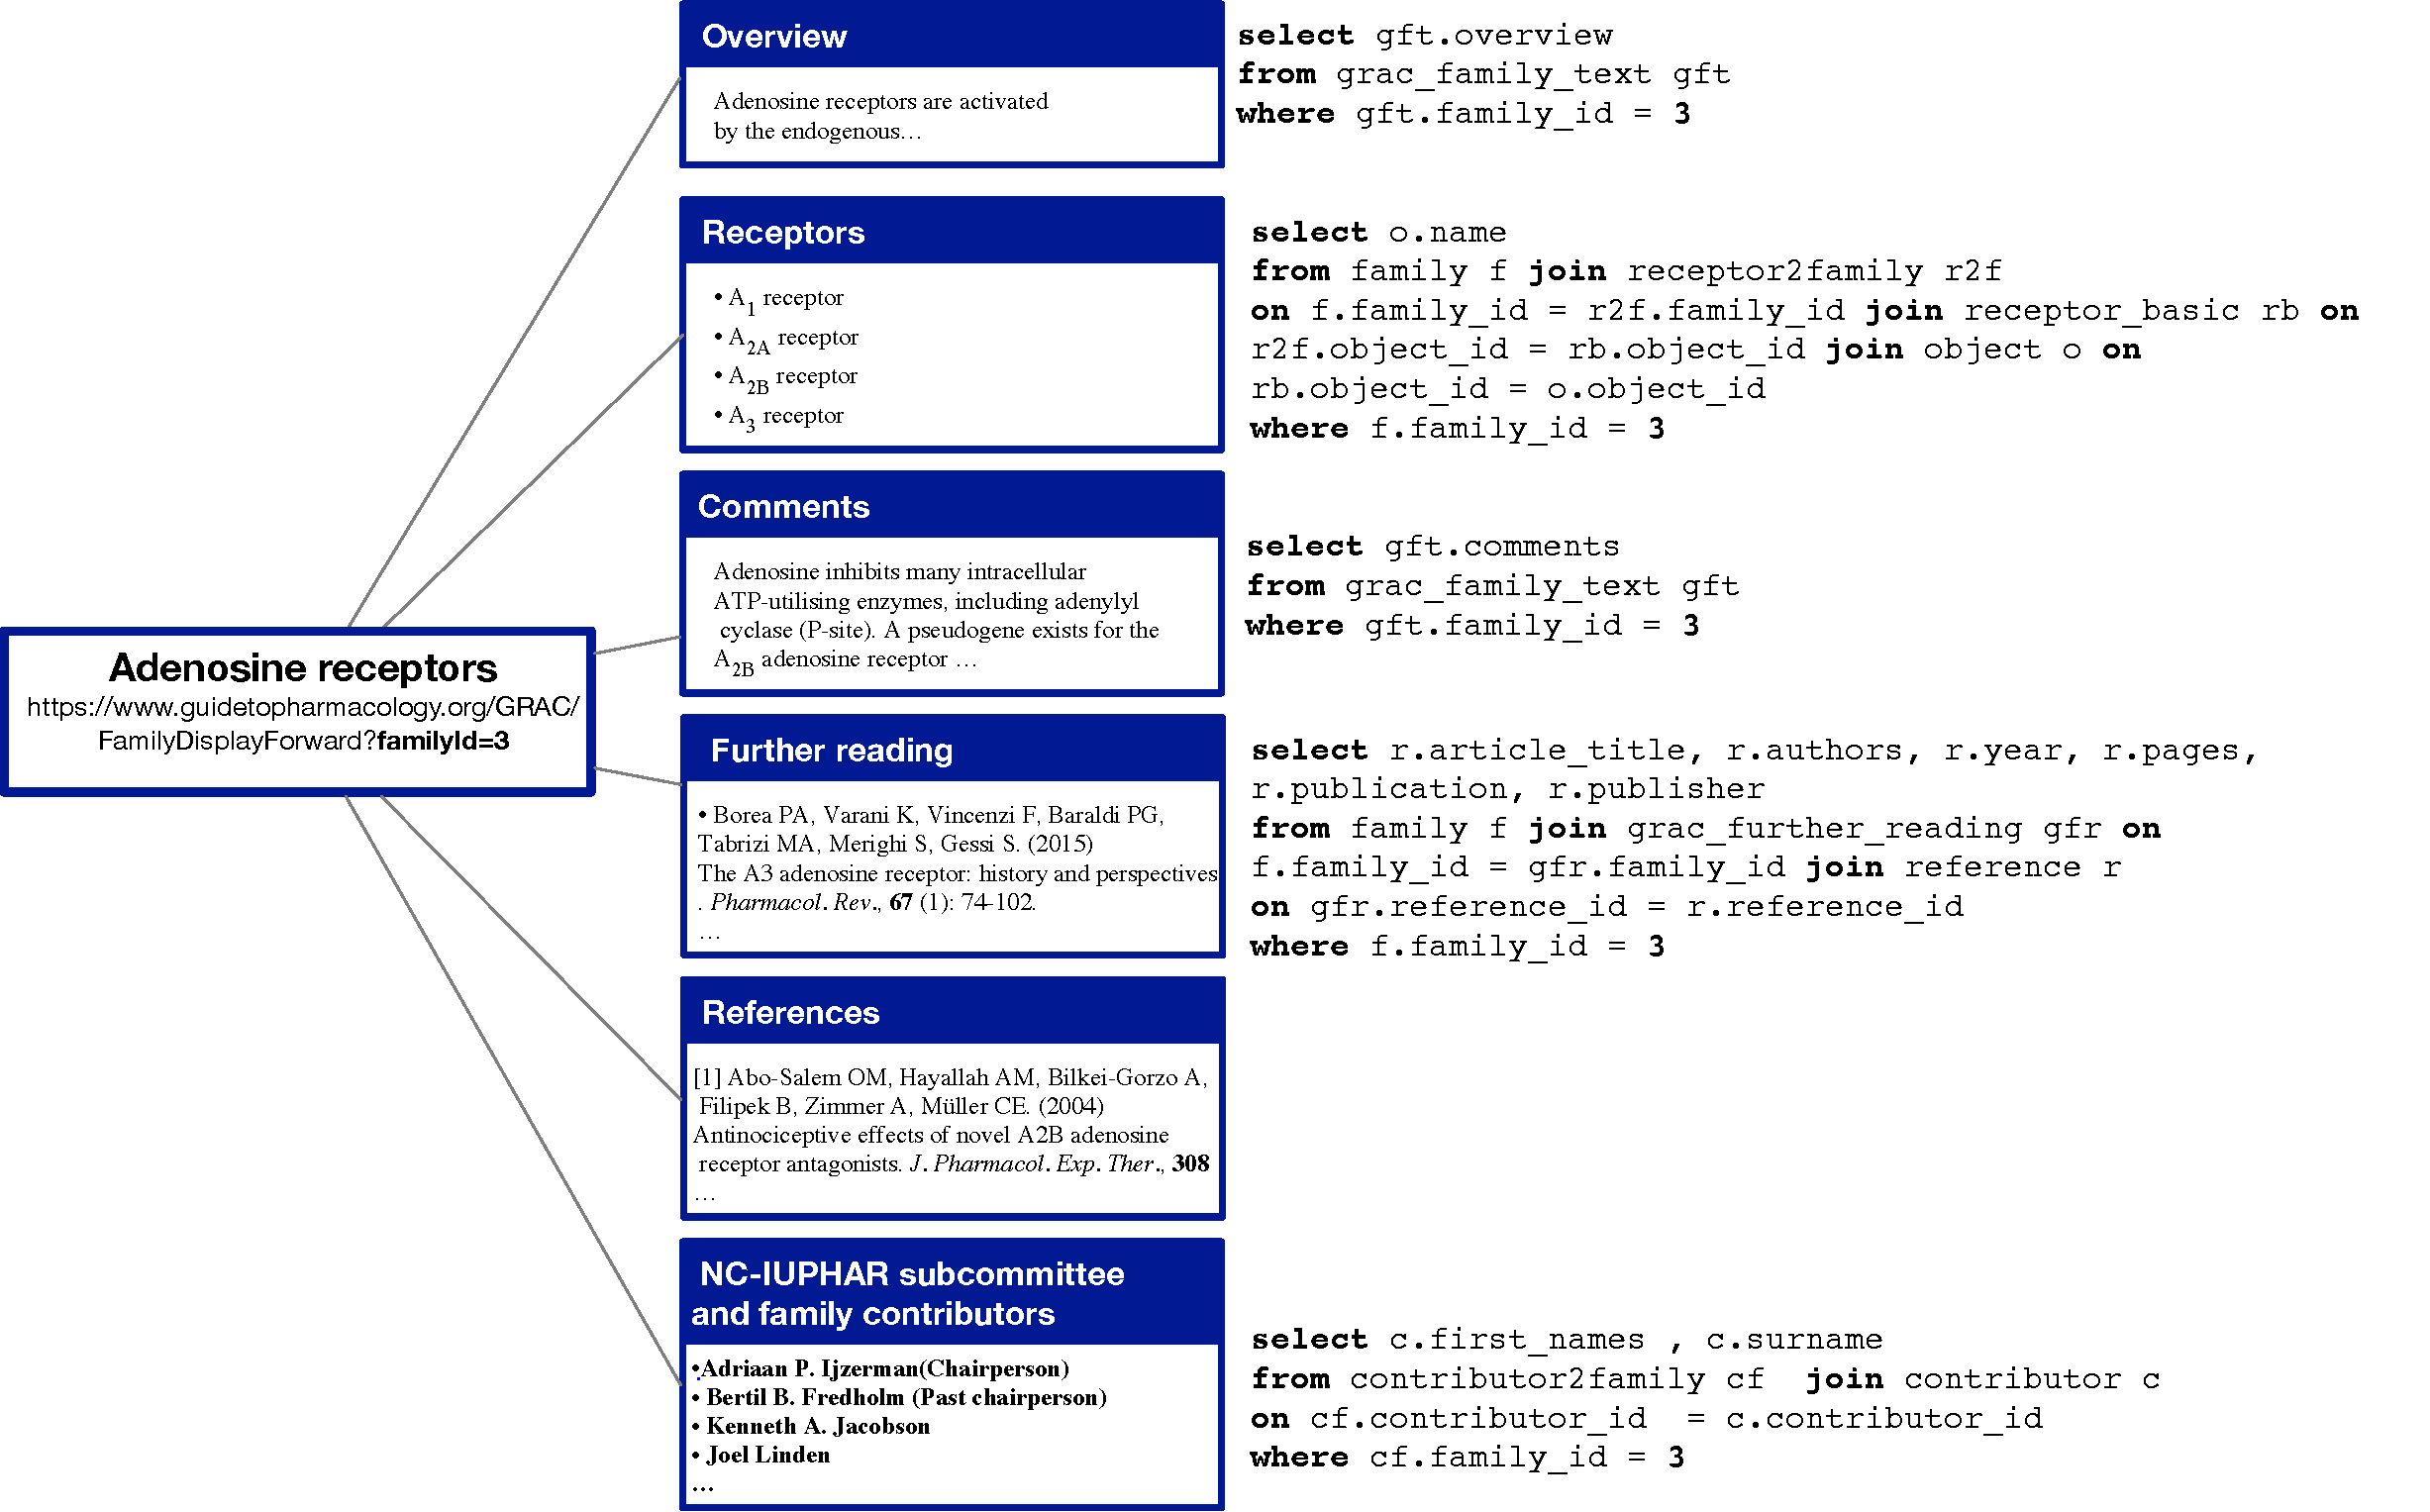
\includegraphics[width=1\textwidth]{figures/family_structure}
  \caption{Basic web-page structure of ``Adenosine receptors'' family (ID 3), with queries used to retrieve the information contained in every section, except references.}
  \label{figure:family_structure}
\end{figure}


GtoPdb provides access to the webpages corresponding to all these nodes through URLs. 
The webpages corresponding to target families all present a similar structure, as shown in Figure \ref{figure:family_structure} for the ``Adenosine receptors'' family. 
Each page has an \emph{Overview}, a brief text describing the content of the page; a list of \emph{Receptors} comprising the family; a section of \emph{comments} about the family;
the \emph{References}, a list of the papers consulted by the curators of the page, similar to a reference list of a paper;
the \emph{further reading} list, reporting papers that an interested reader may want to consult to obtain more insight on the family; and a final section called \emph{How to cite this family page}, containing text snippets useful to cite the specific page or the whole database. 
Figure \ref{figure:family_structure} shows the SQL code that retrieves the information used to build the corresponding sections (apart from the References section).
Therefore, each family page can be considered a full-fledged traditional publication, consisting of title, authors, abstract (the overview), content, and references. 

In practice, many papers in the literature only reference GtoPdb (the root) without including a reference to the specific page being cited. 
That is, they only cite a paper describing GtoPdb as a whole (e.g., \citep{iuphar2018}) and refer to targets, ligands, diseases, etc. only by name. 
Thus, citations to specific families are \emph{de-facto} ``hidden'' to citation systems such as Google Scholar, and useless for the computation of bibliometrics. 

In certain ``lucky'' cases, as with papers available in PDF and published in the British Journal of Clinical Pharmacology~\footnote{\url{https://bpspubs.onlinelibrary.wiley.com/journal/13652125}} (BJCP), when a  family, ligand, receptor name, etc. are used, they have a hyperlink pointing to the corresponding webpage in GtoPdb. Therefore, the citations to the families can be detected and counted using the URLs reported in the papers.
However, these citations to GtoPdb webpages are not counted as such by citation systems, so they are not converted into credit for curators and collaborators. 

For our running example, consider Table \ref{table:running_example}. This simplified version of GtoPdb contains three tables: \texttt{family}, \texttt{contributor} and \texttt{contributor2family}.
% \scream{You have an id column which is "separate" from the other attributes in table.  Are these introduced as provenance tokens, or are they real attributes?  Later you speak about introducing an id in the query result, is this the same?}
The first table, \texttt{family}, has tuples representing families with three attributes: the id of the family, its name, and type. 
Table \texttt{contributor} contains people who have helped generate the data in the database.
The third table, \texttt{contributor2family}, serves as a link between the families and the people who contributed to them.
For instance, ``John Smith'' ($\mathtt{c_1}$) contributed to ``Dopamine Receptors'' ($\mathtt{f_1}$) as well as to the ``YANK Family'' ($\mathtt{f_4}$). Throughout the rest of the paper, we will use the \texttt{id} attribute of these tables as the \emph{provenance token} of its corresponding tuples, that is, as a symbol that serves to identify a tuple when talking about provenance.

\begin{table*}[]
\centering
\begin{tabular}{| l | cc |}
\multicolumn{3}{c}{\textbf{family}}\\
\hline
 id & name & type \\
  \hline
  $f_1$ & Dopamine Receptors & gpcr \\
  $f_2$ & Bile Acid Receptor & gpcr \\
  $f_3$ & FAK Family         & enzyme \\
  $f_4$ & YANK Family        & enzyme \\
\hline
\end{tabular}	
\begin{tabular}{| l |c c|}
\multicolumn{3}{c}{\textbf{contributor2family}}\\
\hline
 id & family\_id & contributor\_id \\
  \hline
  $c2f_1$ & $f_1$ & $c_1$ \\
  $c2f_2$ & $f_1$ & $c_2$ \\
  $c2f_3$ & $f_2$ & $c_3$ \\
  $c2f_4$ & $f_4$ & $c_1$ \\
\hline
\end{tabular}		
\begin{tabular}{| l |c c|}
\multicolumn{3}{c}{\textbf{contributor}}\\
\hline
 id & Name & Country \\
  \hline
  $c_1$ & John Smith & UK \\
  $c_2$ & Jim Doe & UK \\
  $c_3$ & Hans Zimmerman & Germany \\
  $c_4$ & Roberta Rossi & Italy \\
\hline
\end{tabular}		
\caption{Example of a database consisting of three tables. \texttt{family} includes some receptor families in the database; \texttt{contributor} contains the name and country of contributors; \texttt{contributor2family} connects contributors to the families they contributed to.}
\label{table:running_example}
\end{table*}
